\documentclass{article}
\usepackage{amsmath, amssymb, cite, algorithmic, url, braket}
\usepackage{graphicx}
\usepackage{pythonhighlight}
\usepackage[margin=1.5cm]{geometry}
\usepackage[title]{appendix}
\usepackage{subfigure}
\usepackage{listings}
\usepackage{booktabs}
\usepackage{hyperref}

\graphicspath{{../pic/}}
\lstset{
language=[ANSI]{C},
showtabs=true,
tab=,
tabsize=2,
basicstyle=\ttfamily\footnotesize,%\setstretch{.5},
stringstyle=\color{stringcolour},
showstringspaces=false,
alsoletter={1234567890},
otherkeywords={\%, \}, \{, \&, \|},
keywordstyle=\color{keywordcolour}\bfseries,
upquote=true,
morecomment=[s]{/*}{*/},
commentstyle=\color{commentcolour}\slshape,
literate=*%
{=}{{\literatecolour=}}{1}%
{-}{{\literatecolour-}}{1}%
{+}{{\literatecolour+}}{1}%
{*}{{\literatecolour*}}{1}%
{!}{{\literatecolour!}}{1}%
{[}{{\literatecolour[}}{1}%
{]}{{\literatecolour]}}{1}%
{<}{{\literatecolour<}}{1}%
{>}{{\literatecolour>}}{1}%
% {>>>}{\pythonprompt}{3}%
,%
frame=trbl,
rulecolor=\color{black!40},
backgroundcolor=\color{white},
breakindent=.5\textwidth,frame=single,breaklines=true
}

\begin{document}
\title{DSP Homework}
\author{Xu, Minhuan}
\maketitle
\tableofcontents
\begin{abstract}

\end{abstract}

\section{Videos}

\section{How fast do Mosquitoes Flap}
pass

\section{Base-band Wireless Communication Simulate}
\subsection{Simulation and Stability Analysis}
I wrote my code by imitating your code, but I made some changes because I thought there might be a problem with the code in class. This mistake will explain the unstable behavior when noise (along with calculation error) is zero. I wrote my comparison in appendix.

In recovery process, we have
\begin{equation}
	\begin{aligned}
		y &= x * h + n \\ 
		\tilde{y} &= \tilde{x} \times \tilde{h} + N_0 \\
	\end{aligned}
\end{equation}
So, the recovered signal $\hat{x}$ is as below
\begin{equation}
	\begin{aligned}
		\mathcal{F}\{\hat{x}\} &= \tilde{y} \times \frac{1}{\tilde{h}} \\  
		&= ( \tilde{x} \times \tilde{h} + N_0 ) \times \frac{1}{\tilde{h}} \\ 
		&= \tilde{x} + \frac{N_0}{\tilde{h}}
	\end{aligned}
	\label{eq:NoiseInXh}
\end{equation}
Here in (\ref{eq:NoiseInXh}), the IIR $N_0/\tilde{h}$ , is why $\hat{x}$ can be unstable.

\subsection{Unstable Behavior When Noise is Zero}
In mathematics, it is impossible to see unstable behavior in (\ref{eq:NoNoiseXh}).
\begin{equation}
	\begin{aligned}
		\mathcal{F}\{\hat{x}\} &= \tilde{y} \times \frac{1}{\tilde{h}} \\  
		&= ( \tilde{x} \times \tilde{h}) \times \frac{1}{\tilde{h}} \\ 
		&= \tilde{x}
	\end{aligned}
\label{eq:NoNoiseXh}
\end{equation}
So, there must be other noise in the code. What I found is that there will be a very small error in division of python, and it is exactly this little error that makes $1/\tilde{h}$ to oscillate infinitely.

Please see the terminal output in Fig.~\ref{fig:CalculationError} which proves my guess.
\begin{figure}[!h]
	\centering
	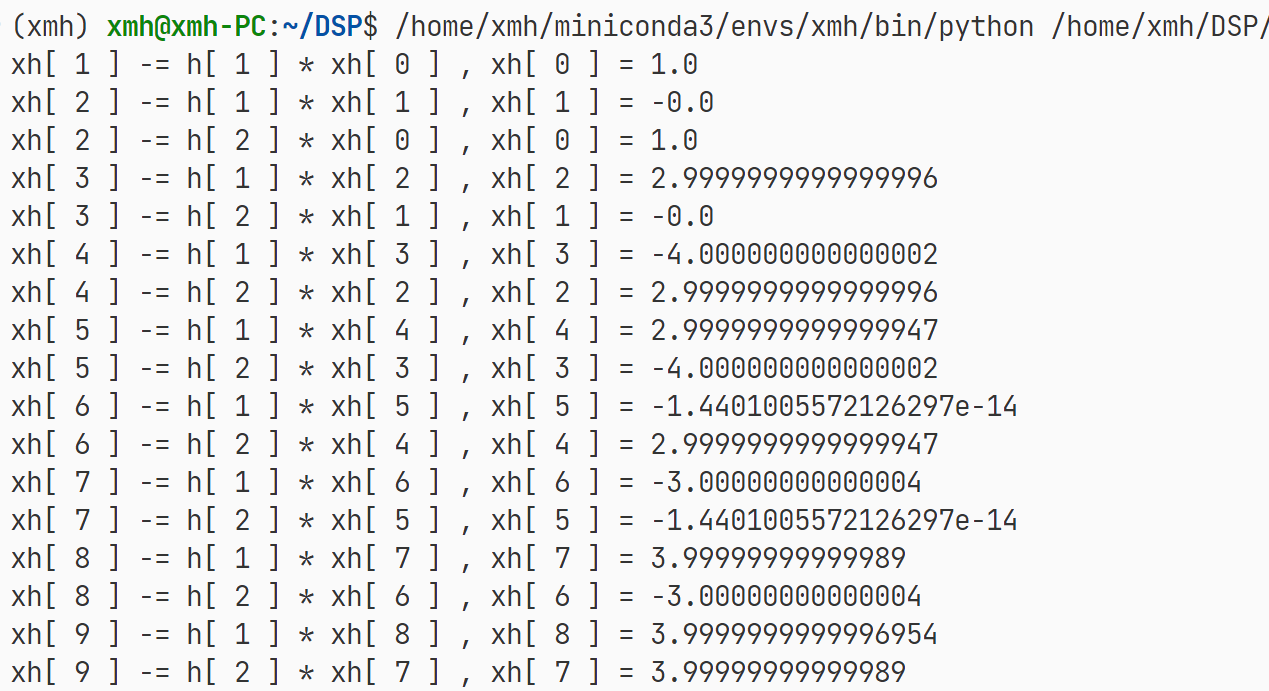
\includegraphics[width=3 in]{../pic/CalculationError.png}
	\caption{Error in Division Calculation}
	\label{fig:CalculationError}
\end{figure}

This error is revealed in float numbers like $2.99\cdots96$ and $-4.00\cdots02$ in line 4 and 6 of Fig.~\ref{fig:CalculationError}.

There are my comparison between whether there is noise or calculation error in signal $y$, see Fig.~\ref{fig:Comparison}.
\begin{figure}[!h]
	\centering
	\subfigure[$\tilde{h}$ is stable]{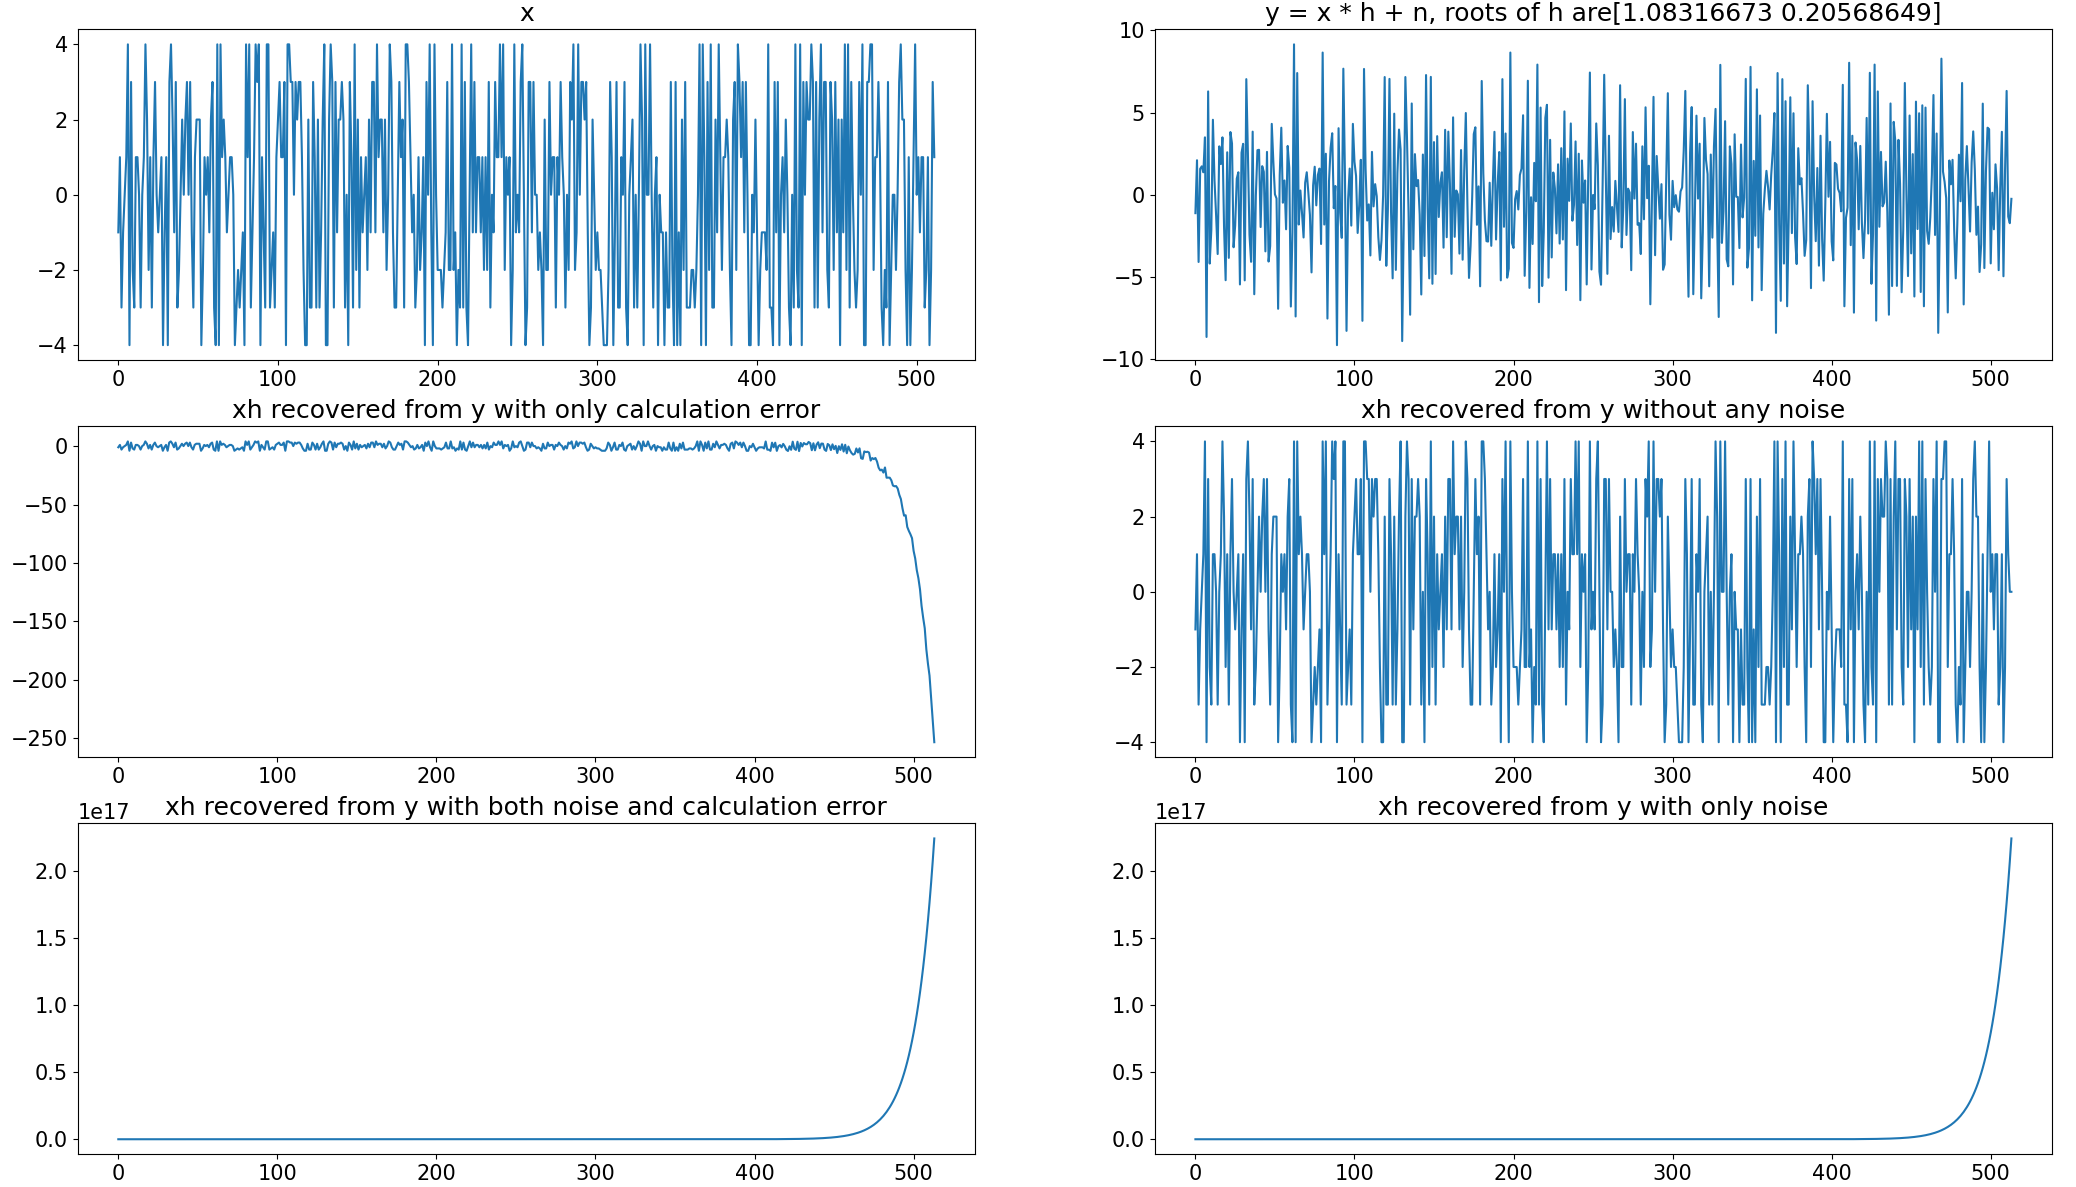
\includegraphics[height=1.7 in]{../pic/StabilityComparison.png}
	\label{fig:StabilityComparison}}
	\hspace{0 pt}
	\subfigure[$\tilde{h}$ is unstable]{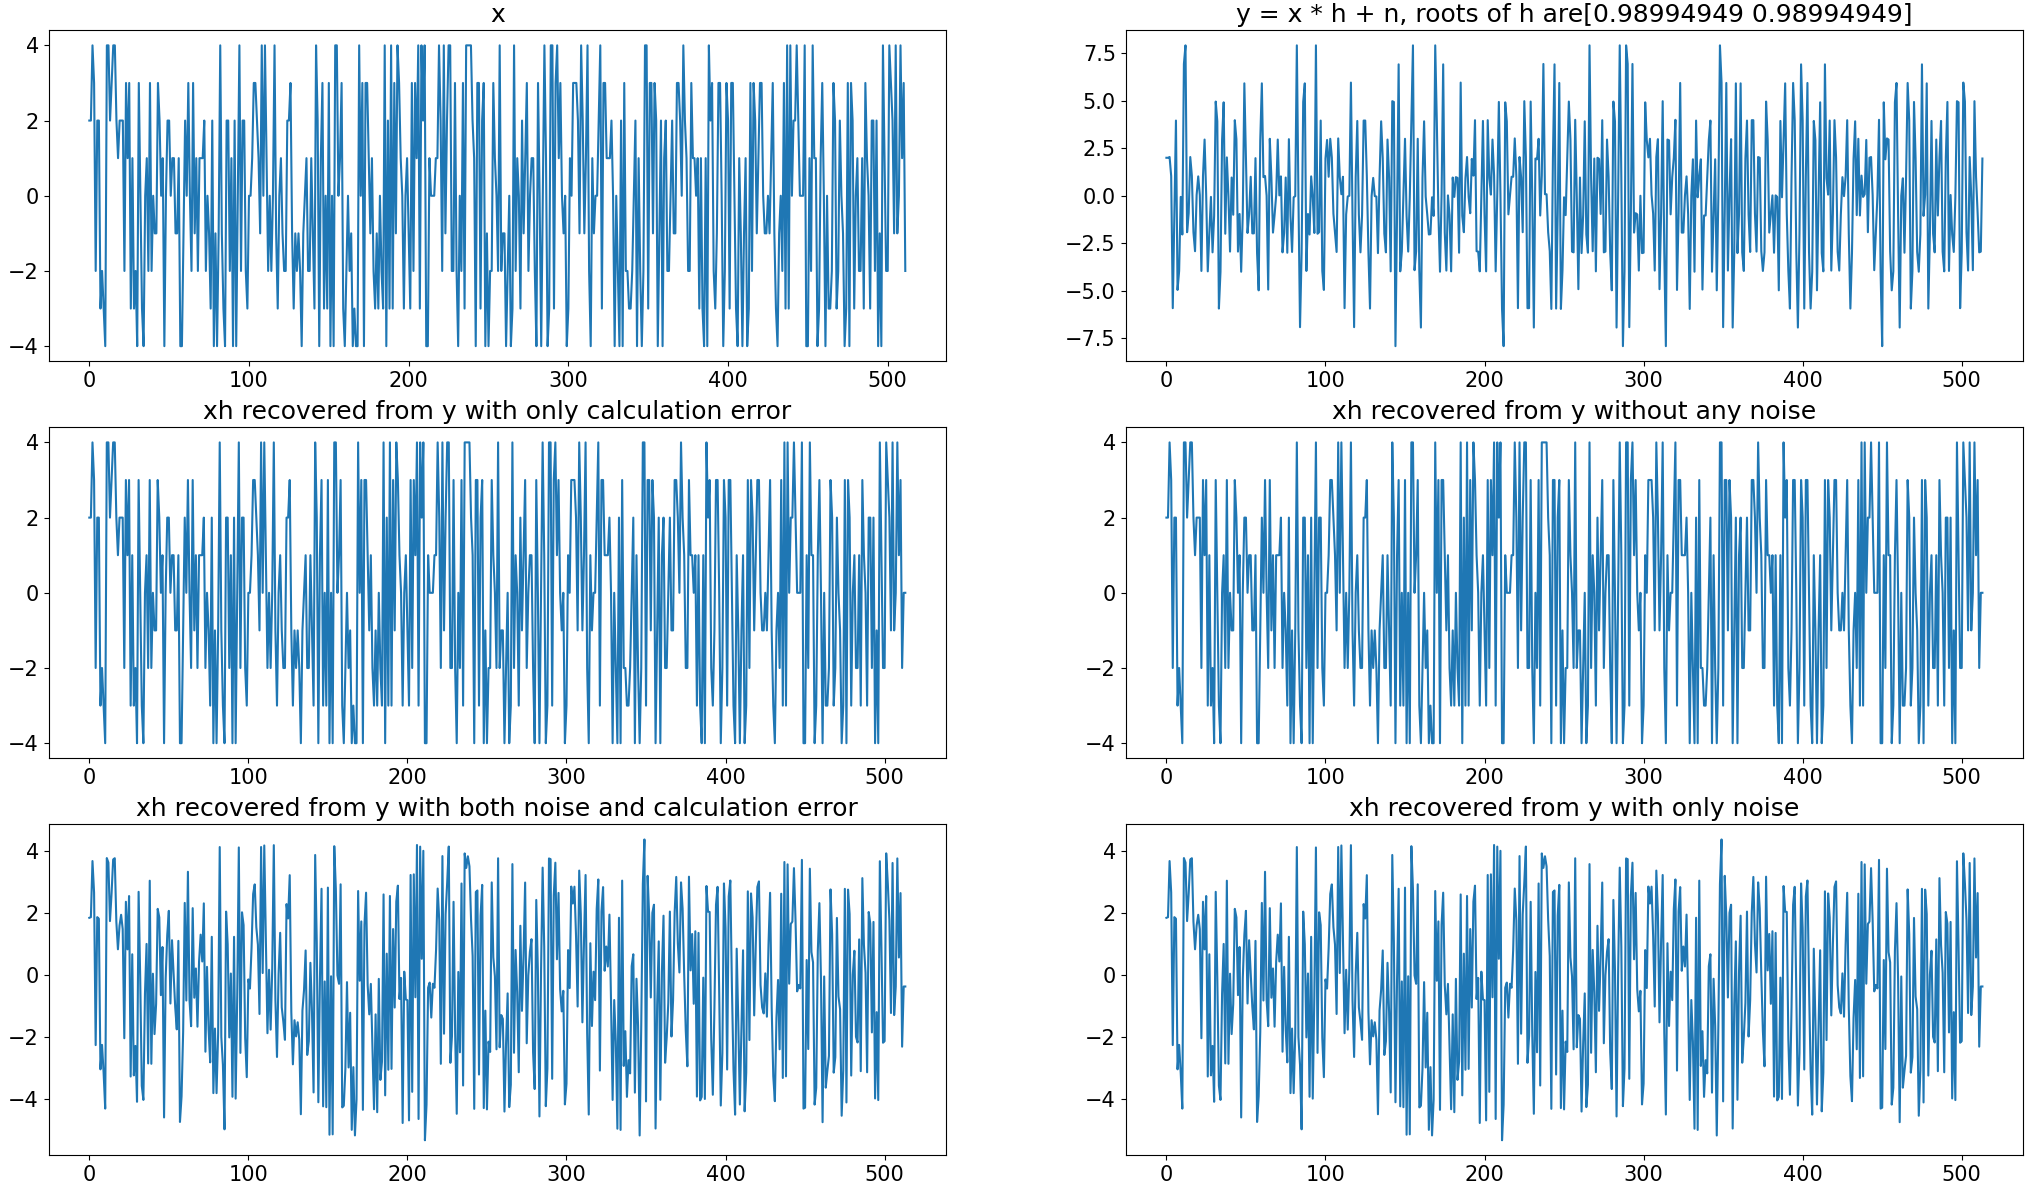
\includegraphics[height=1.7 in]{../pic/AllStableComparison.png}
	\label{fig:AllStableComparison}}
	\caption{Stability Comparison when $\tilde{h}$ is different}
	\label{fig:Comparison}
\end{figure}

We can see in Fig.~\ref{fig:StabilityComparison} that when $\tilde{h}$ is unstable, $\hat{x}$ recovered from y only with calculation error went infinite, but $y$ without both calculation error and noise can be perfectly recovered. This phenomenon is because unstable amplified the noise or the calculation error in recovery, so if there's no disturb in $y$, it is possible to recover the original signal $x$.

Also, when $\tilde{h}$ is stable or is decrement oscillation, the noise and the calculation error will be decreasing along with the recovery process, so without noise is no longer a necessary condition for signal recovery. However, in this condition, only $y$ without any noise can be perfectly recovered ($\hat{x} = x$).

\bibliographystyle{ieeetr}
\bibliography{../bib/database}

\begin{appendices}
\section{Comparison Between Code in Class and My Code}
Dear Yi, I may found a small mistake in your code on Tuesday's class. It is about the recovering of
from $y = x * h$. 

Please see the probably incorrect code as below:
\begin{python}
def reX_estimate(y, h):
	N = len(y)
	M = len(h)
	print("Length of y is ", N,", Length of h is ", M)
	xh = y.copy()
	for n in range(N):
		print("Info: n is now ", n)
		for m in range(1, min(M, n)): # Mistake here, n should be n + 1
			xh[n] -= h[m] * xh[n - m]
			print("xh[", n,"] -= h[",m,"] * xh[",n - m,"]")
		xh[n] /= h[0]
	return xh
\end{python}

The length of $h$ is $3$ and the roots of $h$ are about $[1.77, 0.57]$. Key point is in the output, see Fig.~\ref{fig:output}.

\begin{figure}[!h]
	\centering
	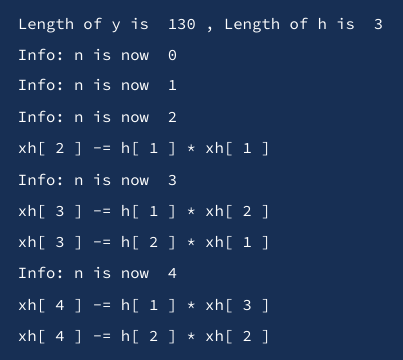
\includegraphics[width=2 in]{../pic/comparisonOutput.png}
	\caption{Output of Test Code}
	\label{fig:output}
\end{figure}

We can find that while $\hat{x}[2] = y[2] = h[0] \times x[2] + h[1]\times x[1] + h[2] \times x[0]$ , this code only minus $h[1] \times x[1]$, that is the small mistake.

This small mistake in recovering $x$ is \emph{working as noise}, as a result, the $h(n)$ which is an unstable IIR, will \emph{amplify this noise} and finally cause the \emph{unstable behavior}. As the Fig.~\ref{fig:diffRec} revealed.

\begin{figure}[!h]
	\centering
	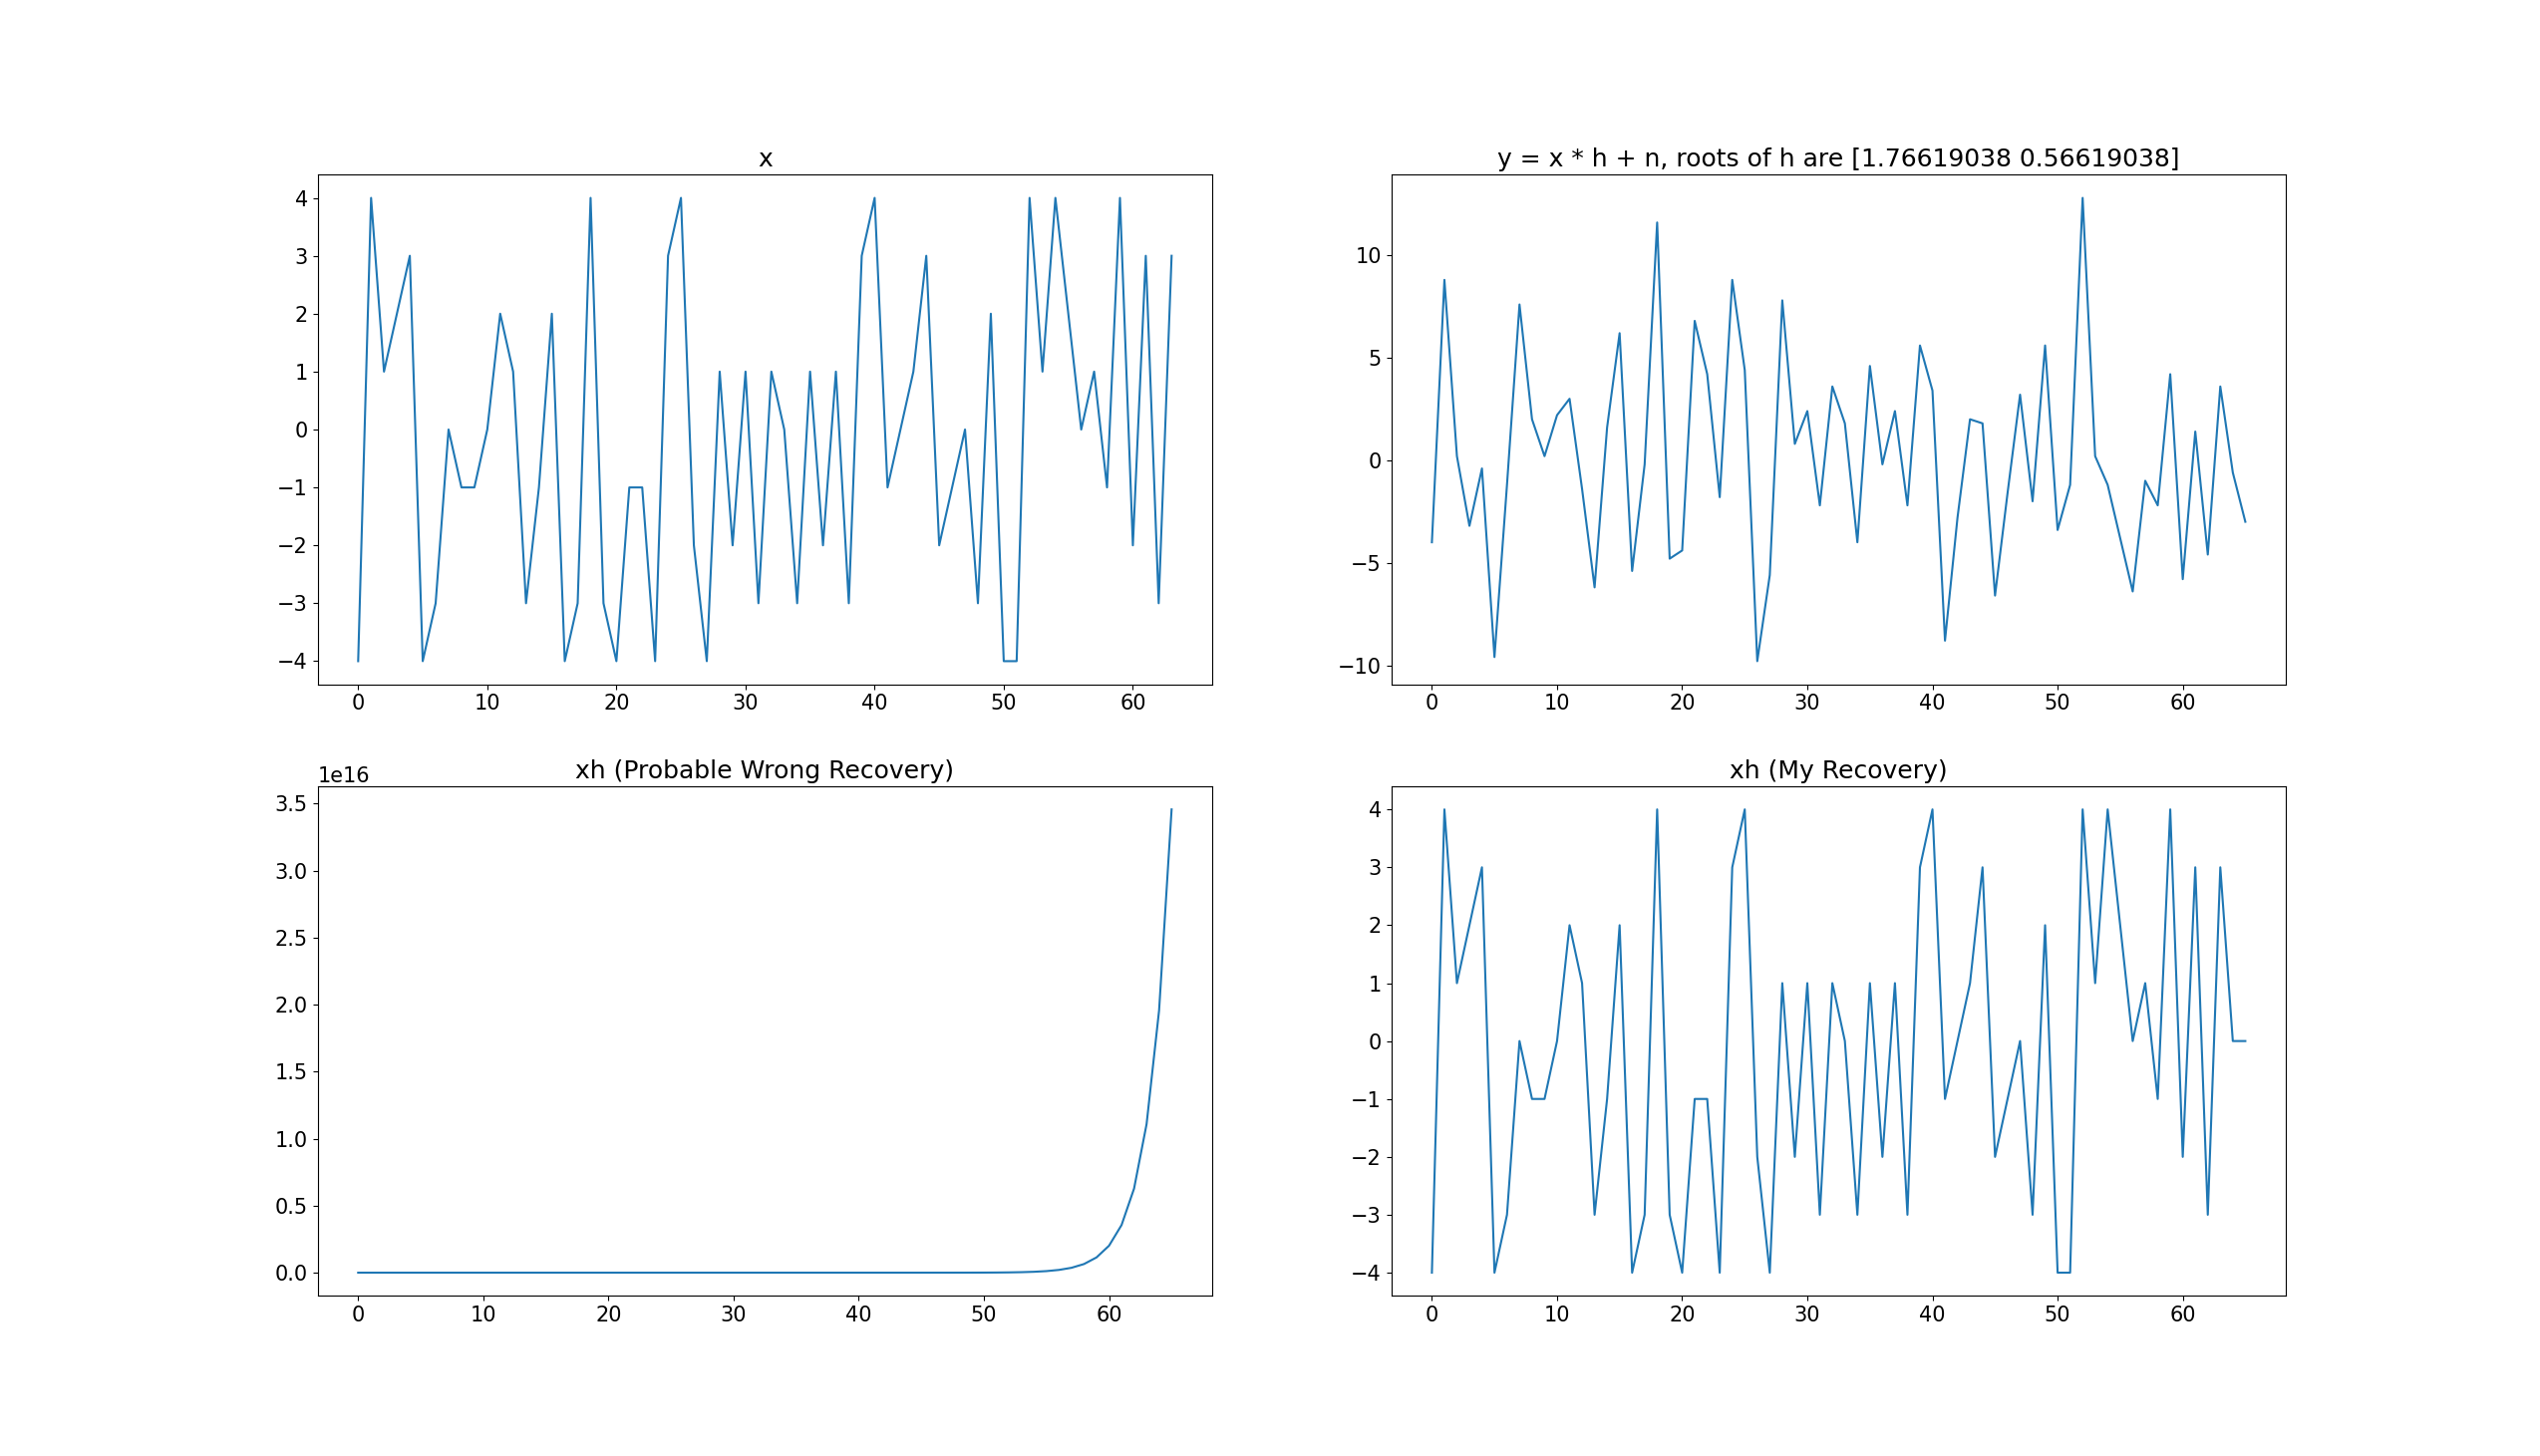
\includegraphics[width=6 in]{../pic/diffRec.png}
	\caption{Different Behavior Between Previous Code and Current Code}
	\label{fig:diffRec}
\end{figure}

% Below is my code for testing.

% \begin{python}
% # test.py
% import numpy as np
% import matplotlib.pyplot as plt
% plt.rcParams.update({'font.size': 15})

% def genPAM(N, M):
%     return (np.random.randint(-M, M + 1, (N)))

% def genNoise(y, snr = 20):
%     Es = np.mean(y**2)
%     sigma = np.sqrt(Es / 10 ** ( snr / 10))
%     n = sigma * np.random.randn(len(y))
%     return n + y, n

% def reX_estimate(y, h):
%     N = len(y)
%     M = len(h)
%     print("Length of y is ", N,", Length of h is ", M)
%     xh = y.copy()
%     for n in range(N):
%         print("Info: n is now ", n)
%         for m in range(1, min(M, n)):
%             xh[n] -= h[m] * xh[n - m]
%             print("xh[", n,"] -= h[",m,"] * xh[",n - m,"]", h[m], xh[n - m])
%         xh[n] /= h[0]
%         xh[n] = np.round(xh[n], 8) #Exclude Error generated by calculation accuracy
%     return xh

% def reX_estimate_new(y, h):
%     N = len(y)
%     M = len(h)
%     print("Length of y is ", N,", Length of h is ", M)
%     xh = y.copy()
%     for n in range(N):
%         print("Info: n is now ", n)
%         for m in range(1, min(M, n + 1)):
%             xh[n] -= h[m] * xh[n - m]
%             print("xh[", n,"] -= h[",m,"] * xh[",n - m,"]", h[m], xh[n - m], xh[n])
%         xh[n] /= h[0]
%         xh[n] = np.round(xh[n], 8) #Exclude Error generated by calculation accuracy
%     return xh

% N = 64
% Nc = 3
% M = 4

% x = genPAM(N, M)
% h = np.random.randn(Nc)
% # h = [1, -1.2, -1]

% y = np.convolve(x, h)
% # y, n = genNoise(y, snr = 30)
% xh = reX_estimate(y, h)
% xh_new = reX_estimate_new(y, h)

% fig = plt.figure(figsize=(12, 8))

% ax = fig.add_subplot(2, 2, 1)
% ax.plot(x)
% ax.set_title('x')
% ax = fig.add_subplot(2, 2, 2)
% ax.set_title('y = x * h + n, roots of h are ' + str(np.abs(np.roots(h))))
% ax.plot(y)
% ax = fig.add_subplot(2, 2, 3)
% ax.set_title('xh (Probable Wrong Recovery)')
% ax.plot(xh)
% ax = fig.add_subplot(2, 2, 4)
% ax.set_title('xh (My Recovery)')
% ax.plot(xh_new)

% plt.show()
% \end{python}

\section{Code Listing}
\begin{python}
# simulate.py
import numpy as np
import matplotlib.pyplot as plt
plt.rcParams.update({'font.size': 15})

def genPAM(N, M):
    """Generate PAM Signal"""
    return (np.random.randint(-M, M + 1, (N)))

def genNoise(y, snr = 20):
    """Generate White Noise"""
    Es = np.mean(y**2)
    sigma = np.sqrt(Es / 10 ** ( snr / 10))
    n = sigma * np.random.randn(len(y))
    return n + y, n

def reX_estimate(y, h, ErrorFlag=1):
    """Estimate x From y"""
    N = len(y)
    M = len(h)
    xh = y.copy()
    for n in range(N):
        # print("Info: n is now ", n)
        for m in range(1, min(M, n + 1)):
            xh[n] -= h[m] * xh[n - m]
            # if ErrorFlag and n <= 20:
            #     print("xh[", n,"] -= h[",m,"] * xh[",n - m,"]", ", xh[", n - m,"] =",xh[n - m])
        xh[n] /= h[0]
        if ErrorFlag == 0:
            xh[n] = np.round(xh[n], 8) #Exclude Error generated by calculation accuracy
    return xh

#parameters
N = 256
Nc = 3
M = 4

#generate x and h randomly
x = genPAM(N, M)
h = np.random.randn(Nc)
# h = [1, 0, -0.98]

#generate y as received signal
y = np.convolve(x, h)
yn, n = genNoise(y, snr = 30) 

#recover x in different methods
xh = reX_estimate(y, h)
xh_new = reX_estimate(y, h, ErrorFlag=0)
xhn = reX_estimate(yn, h)
xhn_new = reX_estimate(yn, h, ErrorFlag=0)

#draw the results and the comparison
fig = plt.figure(figsize=(12, 8))

ax = fig.add_subplot(3, 2, 1)
ax.plot(x)
ax.set_title('x')
ax = fig.add_subplot(3, 2, 2)
ax.set_title('y = x * h + n, roots of h are' + str(np.abs(np.roots(h))))
ax.plot(y)
ax = fig.add_subplot(3, 2, 3)
ax.set_title('xh recovered from y with only calculation error')
ax.plot(xh)
ax = fig.add_subplot(3, 2, 4)
ax.set_title('xh recovered from y without any noise')
ax.plot(xh_new)
ax = fig.add_subplot(3, 2, 5)
ax.set_title('xh recovered from y with both noise and calculation error')
ax.plot(xhn)
ax = fig.add_subplot(3, 2, 6)
ax.set_title('xh recovered from y with only noise')
ax.plot(xhn_new)

plt.show()

\end{python}

\end{appendices}

\end{document}